% Prof. Dr. Ausberto S. Castro Vera
% UENF - CCT - LCMAT - Curso de Ci\^{e}ncia da Computa\c{c}\~{a}o
% Campos, RJ,  2021
% Disciplina: Paradigmas de Linguagens de Programa\c{c}\~{a}o
%


\chapter{Aplicações da linguagem}

Neste capítulo vamos apresentar cinco exemplos de aplicações da linguagem Julia. 

\section{Quicksort}
Um mais importantes algoritmos de ordenação, é inclusive utilizado por padrão na função de ordenação da linguagem \href{https://github.com/JuliaLang/julia/blob/2364748377f2a79c0485fdd5155ec2116c9f0d37/base/sort.jl#L259-L296}{sort!()}. 

Esse algoritmo se inicia elencando um elemento no vetor para ser o pivô dessa execução, a partir de então todos os elementos menores ou iguais ao pivô são colocados antes do mesmo e consequentemente todos os elementos maiores são colocados nas posições seguintes ao pivô. Em seguida é feito uma chamada recursiva da mesma função para cada uma dessas duas porções -do primeiro elemento até o anterior ao pivô, e do elemento seguinte ao pivô até o último. 

No Código \ref{quicksort_code}, apresentamos uma implementação do algoritmo disponível na wiki \href{https://rosettacode.org/wiki/Sorting_algorithms/Quicksort#Julia}{Rosetta Code}. Nela, o mecanismo principal de pivotagem se por meio de duas variáveis que guardam o último elemento da porção inferior ao pivo (left) e o primeiro elemento da porção superior ao pivô (right), ou seja, os limites internos, visto que os limites externos serão os próprios primeiro e último elementos do vetor. Desse modo, essas variáveis dos limites internos se iniciam iguais aos limites externos, se aproximando do pivô da seguinte forma: caso o atual índice left seja menor que o pivo, o índice se desloca mais um elemento a direita, caso o atual índice right seja maior que o pivô ele se desloca para a esquerda, ambas ocorrem até que cheguem em um elemento fora de lugar, e nesse caso o elemento fora de lugar em cada porção são permutados. 
Assim, temos duas porções para abrigarem os elementos maiores e menores que o pivô, que se iniciam vazias, mas vão avançando em direção ao pivô até que englobem todos os elementos. 

Na Fig.\ref{quicksort} implementamos o código no ambiente integrado de desenvolvimento (IDE) \href{https://code.visualstudio.com/docs}{Visual Studio Code} e demonstramos seu funcionamento com um vetor exemplo. 

[TODO: modificar o termo "listing" para algum outro?] 
\begin{lstlisting}[label={quicksort_code},caption={Implementação do algoritmo quicksort em Julia}]
  function quicksort!(A,i=1,j=length(A))
  if j > i
      pivot = A[rand(i:j)] 
      left, right = i, j
      while left <= right
          while A[left] < pivot
              left += 1
          end
          while A[right] > pivot
              right -= 1
          end
          if left <= right
              A[left], A[right] = A[right], A[left]
              left += 1
              right -= 1
          end
      end
      quicksort!(A,i,right)
      quicksort!(A,left,j)
  end
  return A
end
\end{lstlisting}

\begin{figure}[H]
   \begin{center}
       \caption{Quicksort na IDE VScode} \label{quicksort}
       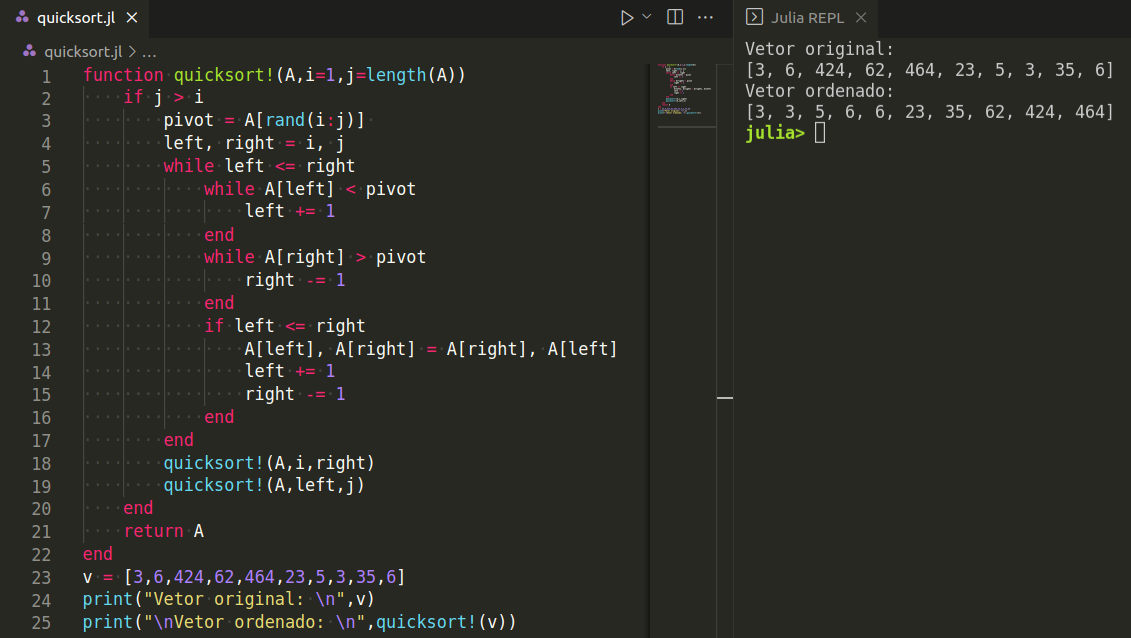
\includegraphics[width=12cm]{aplicacoes/quicksort.png} \\
       {\tiny \sf Fonte: Autor}
   \end{center}
  \end{figure}

\section{Calculadora}
Um aspecto muito importante da computação envolve o uso de interfaces gráficas. Entretanto a construção de janelas, botões e afins é uma tarefa complexa, de modo que na maior parte dos casos os programadores utilizam uma biblioteca que implementa tais componentes de interface gráfica, sendo as duas mais famosas a Qt e a GTK chamadas de GUI Toolkit. 

Nesse exemplo demonstramos uma calculadora simples utilizando a biblioteca Gtk.jl que traz a bilbioteca GTK de forma amigável para a linguagem Julia. 

O código \ref{calculadora_code} apresenta de modo compacto a implementação criada por Nand Vincchi está está disponível como exemplo no repositório \href{https://github.com/JuliaGraphics/Gtk.jl/blob/master/example/calculator.jl}{Github} da biblioteca Gtk.jl. 

Na figura TAL podemos ver o a janela gráfica e parte do código sendo executado na IDE.

\begin{lstlisting}[label={calculadora_code},caption={Calculadora simples em GTK}]
# Simple calculator application that utilises Gtk.jl
# created by Nand Vinchhi for GCI 2019

using Gtk

win = GtkWindow("Calculator")

b1 = GtkButton("1")
b2 = GtkButton("2")
b3 = GtkButton("3")
b_plus = GtkButton("+")
[...]
 
hbox1 = GtkButtonBox(:h)
hbox2 = GtkButtonBox(:h)
hbox3 = GtkButtonBox(:h)
hbox4 = GtkButtonBox(:h)

push!(hbox1, b1)
push!(hbox1, b2)
push!(hbox1, b3)
push!(hbox1, b_plus)
[...]

vbox = GtkBox(:v)
label = GtkLabel("")
GAccessor.text(label,"")

push!(vbox, GtkLabel(""))
push!(vbox, label)
push!(vbox, GtkLabel(""))
push!(vbox, hbox1)
push!(vbox, hbox2)
push!(vbox, hbox3)
push!(vbox, hbox4)
push!(win, vbox)

text = ""

function calculate(s)
	x = "+ " * s
	k = split(x)
	final = 0
	
	for i = 1:length(k)
		
		if k[i] == "+"
			final += parse(Float64, k[i + 1])
		elseif k[i] == "-"
			final -= parse(Float64, k[i + 1])
		elseif k[i] == "x"
			final *= parse(Float64, k[i + 1])
		elseif k[i] == "/"
			final /= parse(Float64, k[i + 1])
		end
	end
	return string(final)
end

function button_clicked_callback(widget)
	if widget == b1
		global text = text * "1"
        GAccessor.text(label, text)
    elseif widget == b2
    	global text = text * "2"
        GAccessor.text(label, text)
    elseif widget == b3
    [...]
        elseif widget == b_equalto
    	global text = calculate(text)
        GAccessor.text(label, text)
    end
end

id1 = signal_connect(button_clicked_callback, b1, "clicked")
id2 = signal_connect(button_clicked_callback, b2, "clicked")
id3 = signal_connect(button_clicked_callback, b3, "clicked")
[...]

showall(win)

\end{lstlisting}


\begin{figure}[H]
   \begin{center}
       \caption{Quicksort na IDE VScode} \label{calculadora}
       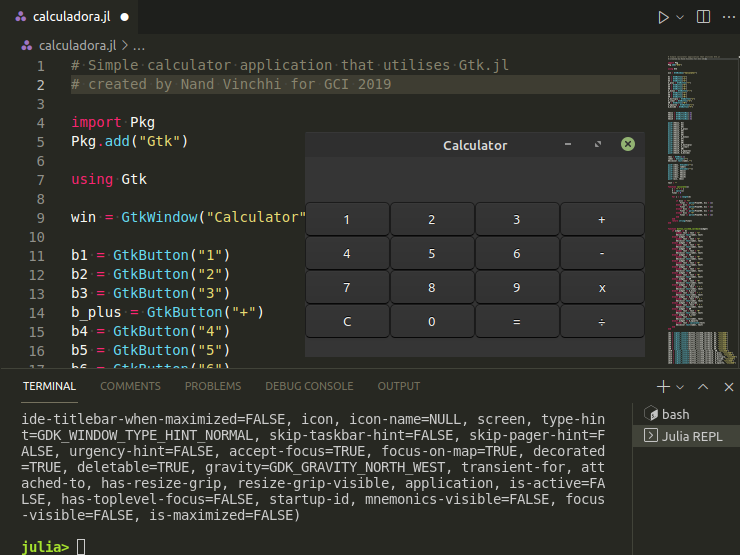
\includegraphics[width=12cm]{aplicacoes/calculadora.png} \\
       {\tiny \sf Fonte: Autor}
   \end{center}
  \end{figure}




